\chapter{Gestaltungsrichtlinien}\label{sec:gestaltungsrichtlinien}

\section{Sprache\index{Sprache} und Textumfag}\label{subsec:sprache_textumfang}

Laut Prüfungsordnung dürfen Bachelor- und Masterarbeiten in deutscher oder englischer Sprache verfasst werden.
Weitere Sprachen sind nach Absprache mit dem Prüfungsausschuss möglich.
Der geeignete Umfang von wissenschaftlichen Arbeiten ist abhängig von Thema, Schreibstil des Verfassers und Anzahl der Verfasser.
Generell sollte man sich an folgenden Richtwerten orientieren.
Die Werte beziehen sich auf den reinen Text ohne Inhaltsverzeichnis\index{Inhaltsverzeichnis}, Literaturverzeichnis oder Anhänge.

\begin{itemize}
    \item{Seminararbeiten ca. 20-30 Seiten}
    \item{Projektdokumentationen ca. 20-40 Seiten}
    \item{Bachelorarbeiten ca. 30-50 Seiten}
    \item{Masterarbeiten ca. 60-80 Seiten}
\end{itemize}

\section{Inhaltliche Bestandteile}\label{subsec:inhaltliche_bestandteile}

Jede Arbeit besteht aus den folgenden Bestandteilen in der vorgegebenen Reihenfolge.
Dabei beginnt jeder Abschnitt auf einer neuen Seite. 

\begin{enumerate}
    \item{Titelseite}
    \item{Inhaltsverzeichnis}
    \item{Abbildungsverzeichnis (optional)}
    \item{Tabellenverzeichnis (optional)}
    \item{Zusammenfassung/Abstract (bei Seminararbeiten und Projektdokumentationen optional)}
    \item{Einleitung}
    \item{Hauptteil}
    \item{Schluss}
    \item{Literaturverzeichnis}
    \item{Erklärung zur Urheberschaft}
    \item{Anhang (optional)}
    \item{Index (optional)}
\end{enumerate}

\minisec{Titelseite}\index{Titelseite}

Die Titelseite enthält alle wichtigen Angaben zu Lehrveranstaltung (Semester, Universität, Lehrveranstaltung, Dozent, Modul), den Titel der Arbeit (im genauen Wortlaut der Themenstellung), Angaben zum Verfasser (Name, Anschrift, E-Mailadresse, Matrikelnummer, Semesterzahl, Datum der Abgabe).
Zusätzlich werden bei Bachelor- und Masterarbeit Erst-und Zweitgutachter angegeben.

\minisec{Inahltsverzeichnis}

Das Inhaltsverzeichnis enthält alle Gliederungspunkte auf allen Ebenen mit den entsprechenden Seitenzahlen.
Es sollen nicht mehr als drei bis maximal vier Gliederungsebenen (1.1.1.1) verwendet werden. Die Nummerierung erfolgt in Dezimalgliederung (1., 1.1 usw.).
Inhaltsverzeichnis und Plagiatserklärung\index{Plagiatserklärung} werden im Inhaltsverzeichnis aufgeführt, aber nicht nummeriert.

\minisec{Einleitung}\index{Einleitung}

Die Einleitung muss nicht zwingend kreativ oder originell sein, sondern ergibt sich aus der Arbeit.
Da sich der genaue Inhalt und die Ergebnisse während der Bearbeitung ändern können, muss die Einleitung eventuell später angepasst werden.
Inhaltlich grenzt die Einleitung das Thema genau ein mit Formulierungen wie „diese Arbeit beschäftigt sich mit XY“.
Danach sollte aufgezeigt werden, inwiefern die Problemstellung für die Medieninformatik relevant ist, sowie die einzelnen Ziele der Arbeit.
Abschließend wird der inhaltliche Aufbau der Arbeit erläutert.
Allgemeinplätze wie „immer mehr Menschen verwenden Computer“ sollten unbedingt vermieden werden.

\minisec{Hauptteil}\index{Hauptteil}

Der Hauptteil beginnt mit einem kurzen Kapitel zu den Zielen der Arbeit.
Bei sehr kurzen Arbeiten, wie einer Seminararbeit, ist dieser Punkt meist mit der Einleitung schon abgedeckt.
Darauf folgt der aktuelle Forschungsstand zum Thema.
Dabei werden unterschiedliche Ansätze vorgestellt und ihre Vor- und Nachteile aufgezeigt.
Je nach Art des Themas fallen die weiteren inhaltlichen Bestandteile unterschiedlich aus.
Im Anhang\index{Anhang} A befinden sich die inhaltlichen Bausteine für eine theoretische, eine konstruktive (Paradigma der „Design Science“) oder eine empirische Arbeit (Paradigma der „Behavioral Science“).

\minisec{Schluss}\index{Schluss}

Im Schlussteil soll deutlich werden, was innerhalb der Arbeit erreicht wurde.
Dazu kann man sich auf die Anfangs beschriebenen Ziele oder Hypothesen beziehen und die wichtigsten Schritte und Erkenntnisse zusammenfassen.
Nach den Ergebnissen kann zusätzlich ein Ausblick gegeben werden, wie sich das Problem weiterentwickeln wird, oder welche weiteren Forschungsfragen sich an die Arbeit anknüpfen.

\minisec{Erklärung zur Urheberschaft}

Eine unterschriebene \emph{Erklärung zur Urheberschaft} ist der Bachelor- und der Masterarbeit beizulegen. Bei der Abgabe von digitalen Arbeiten, z.B. Hochladen einer PDF-Datei auf Grips, reicht die Erklärung ohne Unterschrift aus.
Den konkreten Text der Erklärung finden Sie in der nach dem Anhang.

\minisec{Index}\index{Index}

Bei umfangreichen Arbeiten kann ein Sachwortverzeichnis oder Index sinnvoll sein.
Der Index enthält am Ende der Arbeit bedeutende Schlagworte und dazugehörige Seitenangaben.

\minisec{Anhang}

Material, das innerhalb der Arbeit benutzt wurde oder entstanden ist wie Fragebögen, Nutzungsszenarien, umfangreiche Tabellen, statistisches Datenmaterial, Wireframes oder interaktive Prototypen wird als Anhang ganz zu Schluss der Arbeit beigefügt.
Bei mehreren Anhängen werden diese alphabetisch gekennzeichnet, z. B. „Anhang A Fragebogen“, „Anhang B Nutzungsszenarien“ usw.
Die Anhänge sind im Inhaltsverzeichnis mit aufgeführt aber nicht nummeriert.

Überschaubares Material wie Tabellen, kleinere Mockups, Fragebögen können direkt auf eine Dokumentseite platziert werden.
Umfangreiches Datenmaterial oder interaktive Inhalte können auf einer CD beigefügt werden.
Diese ist dann auf der entsprechenden Seite zu befestigen. 

\section{Formatierung}\label{subsec:formatierung}

\subsection{Seitengestaltung\index{Seitengestaltung} und Druck}\label{subsubsec:seitengestaltung}\index{Druck}

Die Arbeit wird einseitig auf DIN A4 gedruckt. Der Seitenrand beträgt oben 2,5 cm, unten 2,5 cm, links 3, 7 cm, rechts 3,5 cm. Die Kopfzeile enthält die jeweilige Kapitelüberschrift (also die Überschrift erster Ordnung).
Jede Seite, ausgenommen das Deckblatt und das Inhaltsverzeichnis enthält eine Seitennummer mittig in der Fußzeile.
Alle Arbeiten sind in angemessener Weise abhängig vom Umfang zu binden: Für Seminararbeiten genügt ein Schnellhefter oder eine Ringbindung. Für Bachelor- und Masterarbeiten sollte eine Klebe- oder Klemmbindung verwendet werden.

\subsection{Typographie und Textsatz}\label{subsubsec:typographie}

Unterschiede in der Lesbarkeit bestimmter Schrifttypen sind nicht empirisch belegt sondern eher als Faustregeln, die in der typografischen Praxis entstanden sind, zu verstehen:  Serifenschriften wie „Times New Roman“, „Garamond“, „Palatino“ oder „TeX Gyre Pagella“ (wie hier Text)  mit starken Unterschieden in der Strichstärke werden wegen ihrer guten Lesbarkeit häufig bei Texten in Büchern oder Zeitschriften eingesetzt \cite[S.18]{gotz2004typo}.
Serifenlose Schriften wie „Frutiger Next“, „Verdana“ oder „Helvetica“ mit geringen oder keinen Unterschieden in der Strichstärke werden am häufigsten in Titel oder Überschriften verwendet \cite[S.18]{gotz2004typo}. 

  Je nach Schriftart sollte die Schriftgröße für den Fließtext\index{Fließtext} 11- 12pt betragen. Der Zeilenabstand sollte 1,5 fach gewählt werden.

Für die Überschriften \index{Überschriften}kann die gleiche Schrift wie für den Fließtext gewählt werden (wie in der Vorlage) oder man verwendet eine serifenlose Schrift, da sie sich gut von der Serifenschrift im Text abgrenzt.
Beispiele sind „Arial“, die Hausschrift der Uni „Frutiger Next“ uvm.
Bei der Kombination von Schriftarten sollte man grundsätzlich vorsichtig vorgehen und sich an gelungenen Beispielen oder Empfehlungen von Typographen orientieren. 

Für Fußnoten\index{Fußnoten} sollte die gleiche Schrift wie im Fließtext verwendet werden. Die Schriftgröße sollte erkennbar kleiner sein z. B. 10 pt\footnote{Dies ist eine Fußnote}.
Für den Fließtext ist Blocksatz mit automatischer Silbentrennung zu verwenden.
Überschriften aller Art und Verzeichnisse (Literaturverzeichnis etc.) werden linksbündig ausgerichtet.
Zur besseren Lesbarkeit sollte die erste Zeile eines Absatzes eingerückt sein (hier um 0,7cm).
Für eine optimale Seitengestaltung sollte eine vereinzelte Zeile am Anfang einer Seite oder am Ende der Seite (sogenannte „Hurenkinder“ und „Schusterjungen“) vermieden werden.

Zur Hervorhebung von Begriffen können Kursivsetzung oder „Anführungszeichen“ verwendet werden.
Generell sollte man sich für eine Art der Hervorhebung entscheiden und diese dann sparsam und  konsistent verwenden. 

\subsection{Abbildungen}\label{subsubsec:abbildungen}

Abbildungen\index{Abbildungen} werden mit einem Titel und einer Quellenangabe beschriftet.
Ist die Abbildung selbst erstellt oder eine eigene Fotografie so wird dies durch „eigene Abbildung“ bzw. „eigenes Bild“ gekennzeichnet, ein Beispiel ist in Abbildung \ref{fig:abbildung} gezeigt.

\begin{figure}
	\centering
	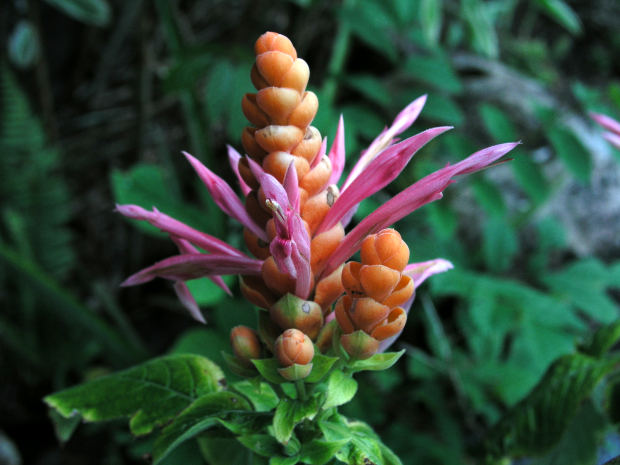
\includegraphics[width=0.5\textwidth]{images/blume}
	\caption{Blumen (Quelle, Jahr, Seitenzahl)}
	\label{fig:abbildung}
\end{figure}

\subsection{Tabellen}\label{subsubsec:tabellen}\index{Tabellen}

{\renewcommand{\arraystretch}{1.5}
\begin{table}[h!]
\centering
\begin{tabular}{ l|l } 
\hline
\bfseries Typ & \bfseries Seitenumfang\\
\hline
Seminararbeit & 20-30 Seiten \\
Bachelorarbeit & 30-50 Seiten \\
Masterarbeit & 60-80 Seiten \\
\hline
\end{tabular}
\caption{Empfohlener Textumfang}
\label{table:textumfang}
\end{table}}

Tabellen sollten nur für Inhalte verwendet werden der auch geeignet ist für eine tabellarische Darstellung wie zum Beispiel der Vergleich von Daten.
Tabellen sind wie Abbildungen mit einer Beschriftung zu versehen.

\subsection{Code\index{Code}}\label{subsubsec:code}

Für Programmcode oder Text in Auszeichnungssprachen wie HTML sollten nichtproportionale Schriftarten wie „Courier New“, „Lucida Console“ oder „Monospace“ verwendet werden.
Die Zeichenbreite ist bei diesen Schriftarten bei jedem Zeichen gleich und die Struktur des Codes ist übersichtlicher.
Generell sollten Codeteile im Hauptteil möglichst kurz gehalten werden, bis ca. 20 Zeilen, da sonst der Lesefluss deutlich unterbrochen wird.
Damit der Programmcode besser lesbar ist und durchsucht werden kann sollte er als Text und nicht als Screenshot eingefügt werden.
Nach Möglichkeit sollte Syntax-Highlighting verwendet werden.
Für die  Erläuterung eines Algorithmus sollte der Code stark vereinfacht und kommentiert werden.


\begin{lstlisting}[language=HTML,caption={So sieht Code schön aus.},captionpos=b,label=code:arduino_blink]
<!DOCTYPE html PUBLIC "-//W3C//DTD XHTML 1.0 Strict//EN"
  "http://www.w3.org/TR/xhtml1/DTD/xhtml1-strict.dtd">
<html xmlns="http://www.w3.org/1999/xhtml" xml:lang="de" lang="de">

<head>
</head>
<body>

</body>
</html>
\end{lstlisting}


\section{Zitierweise}\label{subsec:zitierweise}

Fremde Inhalte, Ideen, Tabellen oder Abbildungen sind über Referenzen im APA-Stil nachzuweisen.
Jede Art von Verweis, direktes oder indirektes Zitat oder der Nachweis von Abbildungen besteht dabei aus einem kurzen Verweis im Text bzw. der Bildbeschriftung und einer vollständigen Auflistung aller Angaben im Literaturverzeichnis.

\subsection{Direkte Zitate}\label{subsubsec:direkte}\index{Direkte Zitate}

Direkte Zitate sind wortgenaue Übernahmen, das heißt, dass jedes Wort so lauten muss wie in der Originalquelle.
Auch grammatikalische oder orthographische Fehler sind zu übernehmen, können aber durch ein nachfolgendes [sic] gekennzeichnet werden.
Kurze Zitate werden in den Fließtext integriert und in „“ gesetzt.
Auslassungen werden mit eckigen Klammern […] sichtbar gemacht.
Auslassungen am Satzanfang werden nicht sichtbar gemacht.
Ein Beispiel: Usability wird definiert als „das Ausmaß, in dem ein Produkt durch bestimmte Nutzer in einem bestimmten Nutzungskontext genutzt werden kann, um bestimmte Ziele effektiv, effizient und zufriedenstellend zu erreichen.“ (DIN EN ISO 9241-11 1997, 94).
Längere Zitate über mehrere Zeilen sollten eingerückt, engerzeilig gesetzt und mit Anführungszeichen dargestellt werden.
Beispiel:

\begin{quote}
«Usability is usually considered the ability of the user to use the thing to carry out a task successfully, whereas user experience takes a broader view, looking at the individual’s entire interaction with the thing, as well as the thoughts, feelings and perception that results from that interaction.»
\cite[S. 4]{albert2013measuring}
\end{quote}

Direkte Zitate sollten sparsam eingesetzt werden, dort wo eine eigene Umschreibung zu einem Bedeutungsverlust oder einer Bedeutungsänderung führt.
Sinnvoll sind direkte Zitate vor allem bei Begriffsdefinitionen oder prägnanten Problemformulierungen.
Beim Zitieren aus fremdsprachigen Originalquellen sollte man keine fremdsprachigen Satzteile  in den deutschen Satz integrieren.
Hier sollte man lieber einen kompletten Satz direkt zitieren oder den benötigten Teil paraphrasieren.

\subsection{Indirekte Zitate}\label{subsubsec:indirekte}\index{Indirekte Zitate}

Indirekte Zitate sind sinngemäße Übernahmen, dass heißt sinngemäße Paraphrasen von Inhalten.
Nach der Umschreibung in einem oder mehreren Sätze folgt die Angabe der Quelle \cite[S. 11]{mustermann2013test}.
Indirekte Zitate dienen dem Beleg von Behauptungen, Methoden oder Fragestellungen in komprimierter Form.

\subsection{Sekundäre Zitate}\label{subsubsec:sekundäre}\index{Sekundäre Zitate}

Wenn der zitierte Inhalt selbst schon ein Zitat ist, handelt es sich um ein sekundäres Zitat.
Im Idealfall sollte ein sekundäres Zitat vermieden und die Originalquelle recherchiert und diese zitiert werden.
Ist die Originalquelle nicht verfügbar, so wird wie folgt referenziert: Zuerst wird die Originalquelle angegeben, danach folgt mit dem Zusatz „zitiert nach“ die Quelle, aus welcher der Inhalt übernommen wurde (\citealp[S. 11]{mustermann2013test}, zitiert nach \citealp[S. 11]{huber2013buch}).

\subsection{Zitierweise im Text}\label{subsubsec:zitierweise}\index{Zitierweise im Text}

Im APA-Stil folgt die Quellenangabe im Text nach dem direkten (Block-) Zitat oder der Paraphrase.
Grundsätzlich sollte die Angabe sobald wie möglich nach der übernommenen Aussage stehen, das heißt nicht erst nach einem ganzen Absatz.
Nachname, Erscheinungsjahr und Seitenangabe werden in runde Klammern gesetzt (Autor, Jahr, Seitenzahl).
Der Zusatz von „Vgl.“ o.ä. ist bei indirekten Zitaten nicht nötig.
Sind keine Seitenangaben verfügbar, so sollten Kapitelüberschriften oder Paragraphennummern verwendet werden.
Wird ein Ansatz oder eine Methode aus einem Aufsatz als Ganzes referenziert müssen keine Seitenzahlen stehen \cite{mustermann2013test}.
Besitzt die Quellenangabe zwei Autoren, so werden beide genannt \cite{mustermann2015gemeinsam}.
Bei drei, vier oder fünf Autoren werden in der ersten Referenz alle genannt \cite*{mustermann2017viele} und bei weiteren Referenzen nur der erste Autor genannt und die anderen mit et al. abgekürzt \cite{mustermann2017viele}.
Die Autorennamen können auch in den Text integriert werden, dann wird nur die Jahreszahl in Klammern angeführt: \citet{mustermann2013test} vergleichen in ihrer Untersuchung.
Bei Wikipedia-Artikeln wird der Titel des Artikels oder die ersten 3-4 Wörter davon in Anführungszeichen angeführt (vor dem letzten Anführungszeichen steht ein Komma \cite{noauthor_wissenschaft_2020}.

\subsection{Angaben im Literaturverzeichnis}\label{subsubsec:angaben}\index{Literaturverzeichnis}

Das Literaturverzeichnis listet alle in der Arbeit referenzierten Quellen in alphabetischer Reihenfolge auf.
Es enthält alle Angaben, die zur Identifikation einer Quelle nötig sind.
Die Vorgaben sind je nach Publikationstyp unterschiedlich.
Die wichtigsten Typen sind unten aufgeführt.
Bei Unklarheiten oder Sonderformen kann im Handbuch der APA nachgeschlagen werden \cite{american2010concise}.

\minisec{Monographie}

% this is needed for bibliography items within the document to work, so nothing to worry about if you don't want to do this
\makeatletter 
\renewcommand\BR@b@bibitem[2][]{\BR@bibitem[#1]{#2}\BR@c@bibitem{#2}}           
\makeatother

\nobibliography*%{literature}
% -------------------------------

\bibentry{sampleMonography}

\bibentry{bortz2007forschungsmethoden}


\minisec{Herausgeberschrift}

\bibentry{sampleCollection}

\bibentry{lewandowski2009handbuch}


\minisec{Artikel oder Kapitel in einer Herausgeberschrift}

\bibentry{sampleInCollection}

\bibentry{butler2002community}


\minisec{Zeitschriftenartikel}

\bibentry{sampleJournalArticle}

\bibentry{schneiderman2002understanding}


\minisec{Beitrag in Konferenzband}

\bibentry{sampleInProceedings}

\bibentry{ehrlich2010microblogging}


\minisec{Elektronische Quellen}

\bibentry{sampleWebsite}

\bibentry{shirky2014ontology}


\minisec{Wikipedia-Artikel}

\bibentry{sampleWikipedia}
